% !TEX program = xelatex

\documentclass[crop,tikz]{standalone}

\usepackage{amsmath}
\usepackage{fontspec}
\setmainfont{CMU Serif}

\usepackage{pgfplots}
\usepgfplotslibrary{fillbetween}

\usetikzlibrary{arrows.meta}
\usetikzlibrary{calc,patterns,angles,quotes}

\pgfdeclarepatternformonly{my crosshatch dots}{\pgfqpoint{-2pt}{-1pt}}{\pgfqpoint{5pt}{5pt}}{\pgfqpoint{11pt}{10pt}}%
{
  \pgfpathcircle{\pgfqpoint{-1pt}{0pt}}{.5pt}
  \pgfpathcircle{\pgfqpoint{4pt}{3pt}}{.5pt}
  \pgfusepath{fill}
}

\begin{document}
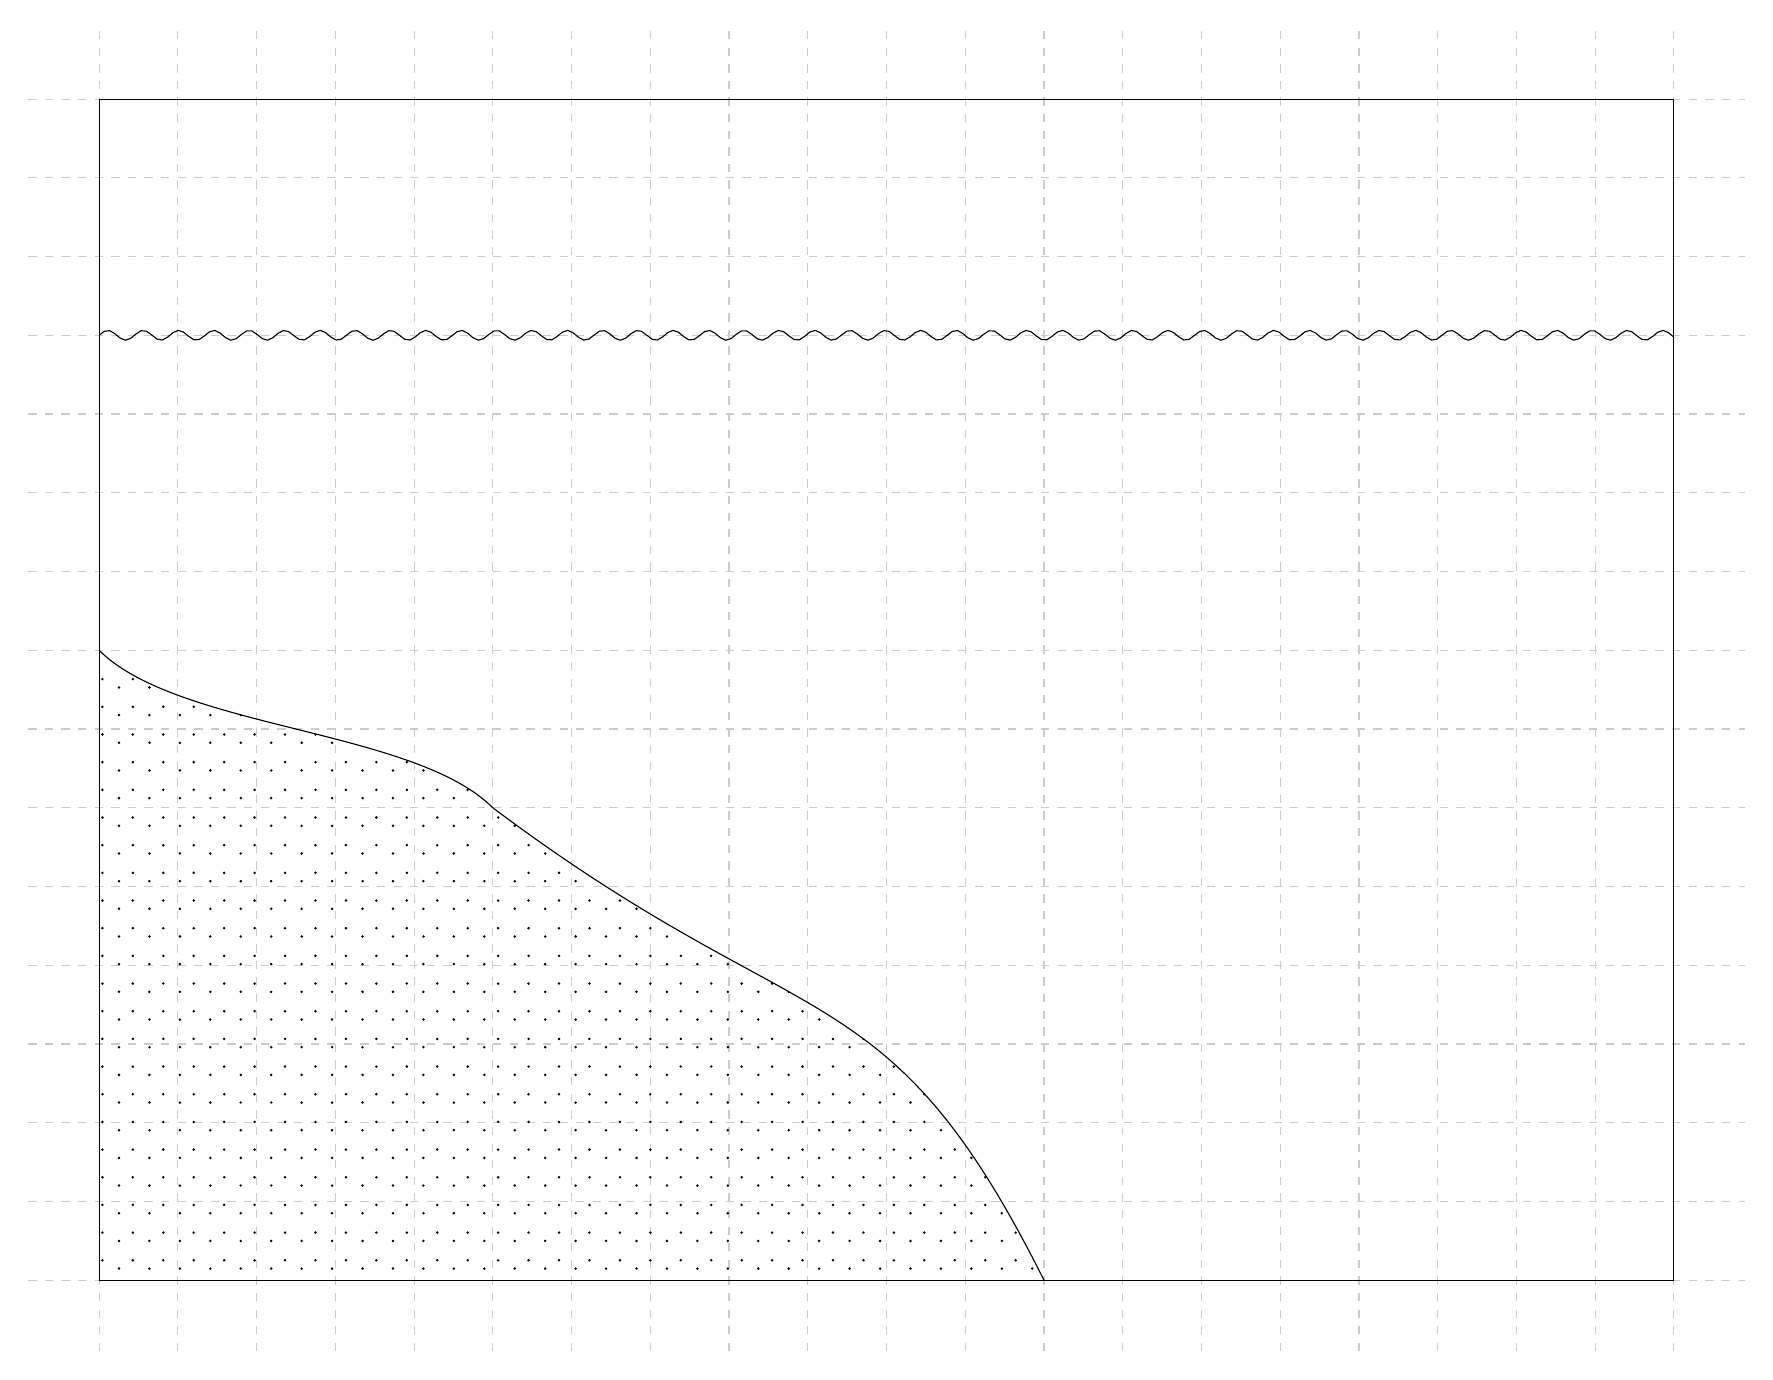
\begin{tikzpicture}[domain=0:20,samples=300]
  \draw[step=1cm,black,thin,opacity=0.2,dashed] (20.9,-0.9) grid (-0.9,15.9);
  
  \draw[name path=land edge] (0,8) -- (0,0) -- (12,0);
  \draw[name path=other edge] (0,8) -- (0,15) -- (20,15) -- (20,0) -- (12,0);
  
  \draw[name path=coast] (12,0) .. controls (10,4) and (9,3) .. (5,6) .. controls (4,7) and (1,7) .. (0,8);
  \tikzfillbetween[
    of=land edge and coast
  ] {pattern=my crosshatch dots};
  
  \draw plot(\x,{sin(14 * \x r) / 16 + 12});
\end{tikzpicture}
\end{document}